\documentclass[a4paper,twoside]{scrbook}
\usepackage{CJKutf8}
\usepackage{url}
\usepackage{biblatex}
\usepackage[colorlinks,linkcolor=red]{hyperref}
\usepackage{graphicx}
\addbibresource{v2pa.bib}
\begin{document}
\begin{CJK}{UTF8}{gbsn}
\title{Volume 2, Part A: P2P Protocols}
\author{EDI}

\frontmatter
\maketitle
\tableofcontents
\mainmatter

\chapter{Introduction}
\section{P2P Technology}
P2P技术属于覆盖层网络(Overlay Network)的范畴,是相对于客户机/服务器(C/S)模式来说的一种网络信息交换方式。在C/S模式中,数据的分发采用专门的服务器,多个客户端都从此服务器获取数据。这种模式的优点是:数据的一致性容易控制,系统也容易管理。但是此种模式的缺点是:因为服务器的个数只有一个(即便有多个也非常有限),系统容易出现单一失效点;单一服务器面对众多的客户端,由于CPU能力、内存大小、网络带宽的限制,可同时服务的客户端非常有限,可扩展性差。P2P技术正是为了解决这些问题而提出来的一种对等网络结构。在P2P网络中,每个节点既可以从其他节点得到服务,也可以向其他节点提供服务。这样,庞大的终端资源被利用起来,一举解决了C/S模式中的两个弊端。
\subsection{NAT穿越技术}
为了缓解网络地址资源日益枯竭的问题,提出了NAT技术用于复用公共IP地址,将网络划分为了内外网,这导致不在同一个内网中的客户端无法直接通信。基于C/S架构的通信模型需要内网的客户机主动向服务器发起连接请求,服务端不能主动发起对内网的请求,而参与P2P的双方互为客户机和服务器,因此两者无法建立起直接通信,为了解决这一问题,需要使用NAT穿越技术。包括1。应用层网关(ALG) 2.中间件技术(uPNP) 3.打洞技术 4、Relay服务器中转技术。经过NAT穿越后可以建立起两个节点的通信通道,双方可以直接交换数据。
\subsection{P2P网络结构}
P2P网络有3种比较流行的组织架构,包括DHT结构、树形结构、网状结构,根据应用的需求可以灵活采用不同的结构或者把它们混合使用。

1.DHT结构

分布式哈希表(DHT)是一种分布式存储方法。虽然DHT具有各种各样的实现方式,但是具有共同的特征,即都是一个环行拓扑结构,在这个结构里每个节点具有一个唯一的节点标识(ID),节点ID是一个128位的哈希值。每个节点都在路由表里保存了其他前驱、后继节点的ID。如图\ref{fig:P2P network architecture}(a)所示。通过这些路由信息,可以方便地找到其他节点。这种结构多用于文件共享和作为底层结构用于流媒体传输。

2.树形结构

P2P网络树形结构如图\ref{fig:P2P network architecture}(b)所示。在这种结构中,所有的节点都被组织在一棵树中,树根只有子节点,树叶只有父节点,其他节点既有子节点也有父节点。信息的流向沿着树枝流动。最初的树形结构多用于P2P流媒体直播。

3.网状结构

网状结构如图\ref{fig:P2P network architecture}(c)所示,又叫无结构。顾名思义,这种结构中,所有的节点无规则地连在一起,没有稳定的关系,没有父子关系。网状结构为P2P提供了最大的容忍性、动态适应性,在流媒体直播和点播应用中取得了极大的成功。当网络变得很大时,常常会引入超级节点的概念,超级节点可以和任何一种以上结构结合起来组成新的结构,如KaZaA\cite{leibowitz2003deconstructing}。

\begin{figure}[!htbp]
\centering
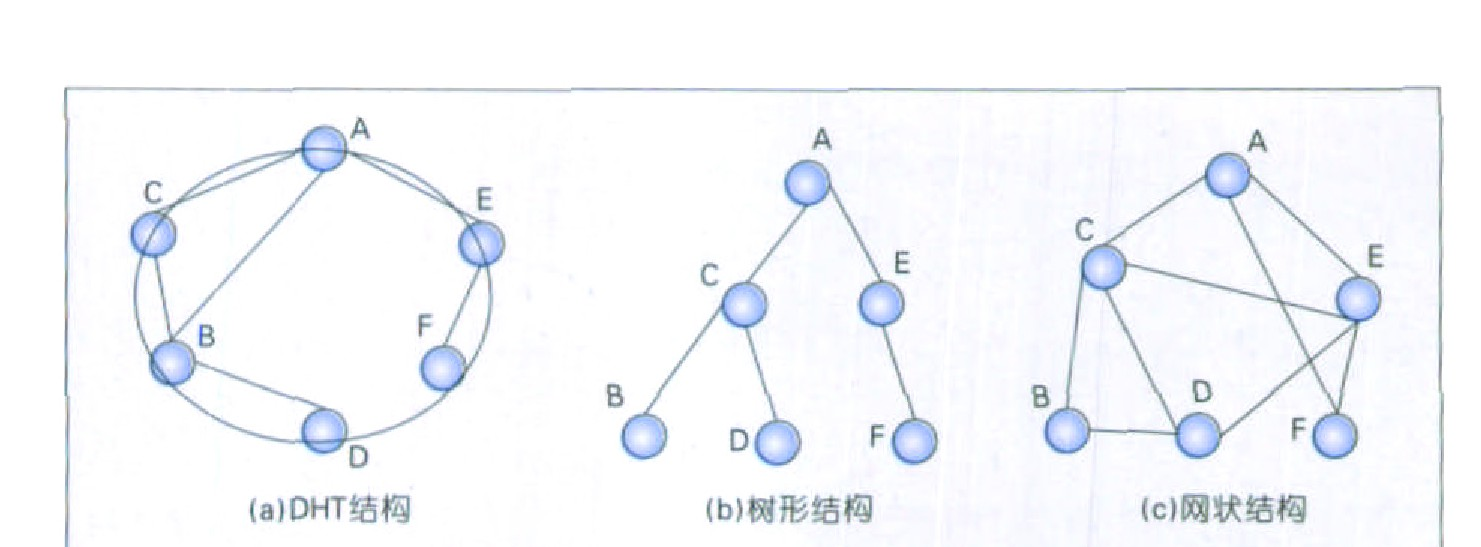
\includegraphics[width=1\textwidth]{Figures/P2P network architecture.png}
\caption{P2P网络结构分类图} 
\label{fig:P2P network architecture}
\end{figure}

\subsection{P2P应用}
P2P技术可以解决传统架构中服务器端带宽瓶颈和节点失效的问题,充分利用客户机的剩余资源,因此P2P技术被广泛地应用于计算机网络的各个领域中,包括文件共享、流媒体传输、分布式计算、即时通讯、区块链、物联网等。
1.文件共享:P2P 技术最初就是应用于文件共享,用户可以共享和下载各种类型的文件,如音乐、电影、软件等。1999 年,Napster 推出了一款点对点音乐共享软件,允许用户直接共享和下载音乐文件。这是 P2P 技术的第一个成功应用,开启了点对点文件共享的时代。随后,Gnutella 推出了一个开源的 P2P 文件共享网络,进一步推动了 P2P 技术的发展。

2.流媒体内容分发:P2P 技术可以构建内容分发网络,实现高效的文件分发和传输,比如实现高效的流媒体传输。学术界的研究内容包括但不限于负载均衡策略、缓存替换算法、内容分发算法等。工业界的成功案例包括PPLive、PPStream、沸点和TVAnts等,

3.即时通讯:P2P 技术允许用户直接进行点对点通信,实现实时的文本、语音和视频通讯。比如ICQ,QQ,MSN Messenger,Yahoo通等即时通信软件,还有以Skype为代表的语音通信软件。

4.分布式计算:P2P 网络可以利用网络中多个节点的计算能力,实现分布式计算,例如科学计算、机器学习等。这种计算一般是计算量巨大、数据极多、耗时很长的科学计算。在每次计算过程中,任务(包括逻辑与数据等)被划分成多个片,被分配到参与科学计算的P2P节点机器上。在不影响原有计算机使用的前提下,人们利用分散的CPU资源完成计算任务,并将结果返回给一个或多个服务器,将众多结果进行整合,以得到最终结果。

5.区块链:区块链是一种基于 P2P 网络的分布式账本技术,它为各种应用提供了安全、透明和不可篡改的交易记录。比特币和以太坊等数字货币都实现了属于自己的P2P网络协议。这些协议使得节点可以安全地交换数据,验证交易的有效性,并达成共识。

5.物联网:随着移动设备普及,传统的NVR方案已经无法满足随时随地就可以访问物联网设备采集到的实时视频和历史录像。而视频数据全部上云的方式又会带来极高的成本。P2P 技术可以应用于物联网领域,实现设备之间的直接通信和数据共享。

\subsection{P2P协议分类}
1.中心化P2P网络:中心服务器对于中心化网络结构至关重要,保存接入节点的地址信息是网络的核心。普通节点通过接入中心服务器获取其他节点地址,从而实现节点与节点之间的通信。早期MP3共享软件Naspter采用的就是中心化网络结构。将音乐文件与保存文件的节点相互关联,用户查找某个音乐时,中心服务器告知储存节点地址,用户点对点连接以获得音乐。中心服务器也决定着网络整体稳定性,一旦中心服务器出现问题,整个P2P网络就会瘫痪。

2.全分布式非结构化P2P网络: 全分布P2P节点可以自由加入、退出,并且没有中心节点,节点地址没有结构化统一标准,整个网络结构呈随机图的结构,无固定网络结构图。其成功的应用产品是gnutella通信协议,它是一种点对点的搜索系统。gnutella采用的是洪泛(flooding)技术实现发现其他节点和随机转发的机制,采用 TTL(timetolive)的减值来实现控制消息通信有限次数传播。然而完全的自由意味着新节点无法得知P2P网络节点信息,从而无法加入网络。因此 gnutella使用了目录服务器来方便节点得到其他节点的网络地址。全分布式P2P网络更加自由化的同时也带来了节点管理的问题,节点频繁地加入/退出使得整个网络结构无法稳定,大量的广播消息不仅造成资源浪费,甚至会阻塞网络。中本聪设计的比特币采用的就是这种P2P网络结构,全分布式使得任何人任何节点都可以参与,非结构化使得节点间既可以通过区块链P2P协议同步区块数据,又保持匿名隐私保护,使得区块链分布式去中心化概念深入人心。

3.全分布式结构化P2P网络:全分布式最大的问题在于节点地址管理,节点间没有固定规则约束,无法精确定位节点信息,只能通过洪泛查询的方式进行查找,对网络的消耗很大。结构化网络采用分布式哈希表(distributedhashtable,DHT),通过如 hash函数一类的加密散列函数将不同节点地址规范为标准长度数据,比较成功的案例有eMule及其Kademlia 网络。网络结构与非结构化相同,都是随机形式、无固定结构,但节点管理有固定结构图。以太坊将节点椭圆加密算法的公钥转换为 64 Byte的 nodeId作为唯一标志符来区分节点,使得以太坊可以在没有中心服务器的情况下实现节点地址的精确查找。

4.半分布式P2P网络:结合中心化和分布式模型各自的优点,将节点分类成普通节点和超级节点,从而构成了半分布式网络结构。每个超级节点维护部分网络节点地址、文件索引等工作,超级节点共同实现中心服务器功能。超级节点本身却是分布式的,可以自由扩展退出,具备分布式网络优点,kazza是其代表性的成功应用。超级账本(fabric)采用的 P2P网络结构就是半分布式,将节点分为普通用户节点和超级节点(排序、背书节点等)。超级节点可以由普通节点选举,也可以自行配置,单独一个超级节点停机不影响系统运行。超级账本所有交易必须通过超级节点认证,区块也是由超级节点生成,普通节点间可以互相同步区块。

\url{https://javaforall.cn/184333.html}
\subsection{BitTorrent}
布拉姆·科恩 (Bram Cohen)于 2001 年设计了 BitTorrent 协议。科恩用 Python 编写了第一个客户端实现。BitTorrent 是一种文件共享方式,使用 BitTorrent 共享的文件被分成更小的部分,分发给协议的用户,这些用户被称为peer,允许其他peer进行搜索并下载他们的文件副本,这使得Bittorrent可以在较低的带宽下高效工作。

BitTorrent 客户端的第一个版本没有搜索引擎,也没有对等交换,想要上传文件的用户必须创建一个小型的torrent 描述符文件,然后将其上传到 torrent 索引站点。当用户想要共享文件时,他们会为文件做种。这个用户被称为做种者。他们将一个 torrent 描述符文件上传到交换器(我们稍后会讨论这一点)。任何想要下载该文件的人都会下载这个 torrent 描述符。但是,BitTorrent 也可以在没有种子的情况下工作;一组对等点可以共享文件的片段,只要他们之间拥有原始完整文件的所有片段。一些跟踪器网站通过惩罚在下载完成后不播种文件的对等点来鼓励播种。

BitTorrent的关键元素包括Swarm和Tracker。Swarm是正在下载或上传内容的机器社区。Tracker是一种专用工具,功能类似于搜索引擎。但是,它会跟踪集群中包含的文件,并允许用户查看以及快速访问他们可能需要的任何文件。要访问 Swarm 和 Tracker,必须先下载 BitTorrent 客户端。在计算机上安装该客户端后,即可查找和下载文件。

自从Bittorrent提出以来,用 Torrent 作为搜索引擎的新网站开始流行起来。比如,海盗湾运营着最受欢迎的Tracker之一,直到 2009年因侵犯版权被禁用,运营人员被判入狱并被处以罚款;但此后,该网站仍在运营,并且终止Tracker,全面转向DHT协议,现在非常受欢迎,每天吸引约三百万访问者。DHT为我们提供了类似字典的界面,但节点分布在网络中。DHT通过对magnet字符串进行哈希处理,可以找到存储特定密钥的节点,这实际上使每个peer都成为一个微型Tracker。

兼容Bittorrent协议的客户端如图\ref{fig:Bittorrent}所示。
\begin{figure}[!htbp]
\centering
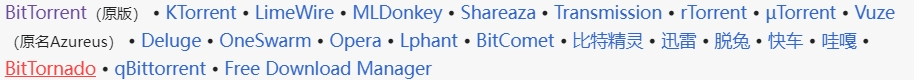
\includegraphics[width=1\textwidth]{Figures/Bittorrent.png}
\caption{Bittorrent协议的客户端} 
\label{fig:Bittorrent}
\end{figure}


\url{https://skerritt.blog/bit-torrent/#%F0%9F%98%8E-optimistic-unchoking}

\url{https://www.britannica.com/technology/BitTorrent}

\url{https://visual.ly/community/Infographics/technology/history-bittorrent}

\subsection{eMule}
在2002年5月13日的黎明,一个叫Merkur的人对原始的eDonkey2000客户端感到不满,他坚信他能做的更好。他在自己的周围聚集了很多的开发人员,eMule工程也由此诞生。他们的目标是将eDonkey的精华保留下来,增加新的功能,并使图形界面更加友好。他们无法想象此时的决定会带来什么样的影响……

今天,eMule网络由数百台eMule服务器和数百万个eMule客户端组成。客户端应该连接一台服务器以获得网络服务,只要客户端在系统中,服务器连接就会保持打开状态。服务器执行集中式索引服务,并且不与其他服务器通信。每个eMule客户端都预先配置了服务器列表和本地文件系统上的共享文件列表。客户端使用与eMule服务器的单一TCP连接登录网络,获取所需文件和可用客户端的信息。eMule客户端还使用数百个TCP连接到其他客户端,这些客户端用于上传和下载文件。每个eMule客户端都为其共享文件维护一个上传队列。下载客户端在队列的底部加入队列并逐渐前进,直到它们到达队列的顶部并开始下载他的文件。客户端可以从其他几个eMule客户端下载相同的文件,从每个客户端获得不同的片段。客户端还可以上传尚未完成下载的文件块。最后,eMule扩展了eDonkey功能,允许客户端交换有关服务器、其他客户端和文件的信息。请注意,客户端和服务器通信都是基于TCP的。

eMule服务器不存储任何文件,它充当存储文件位置信息的集中索引。服务器的另一个功能是在通过防火墙连接但无法接受传入连接的客户端之间进行桥接,这一功能已被弃用。桥接功能大大增加了服务器负载。eMule使用UDP来增强客户端对抗服务器和其他客户端的能力。客户端发送和接收UDP消息的能力对于客户端的正确日常操作不是强制性的,当防火墙阻止它发送和接收UDP消息时,它将完美地工作。

eMule能够连接eDonkey和Kademlia两个网络,有较快的下载损坏数据恢复功能,拥有eD2k Hash验证和AICH损坏文件智能恢复,保证了最终下载的文件将和上传者上传的文件完全一致。AICH全名Advanced Intelligent Corruption Handling(高级智能型损坏处理),是智能型损坏处理(Intelligent Corruption Handling)的加强版。AICH是文件共享软体(eMule,aMule)使用的一种用以确保文件在网络传输时没有错误的方法。万一错误发生,称为“损坏”,AICH运算法以最小的额外重新下载资料量来修正这个损坏。与Bittorrent协议不同,eMule采用客户积分的方式,对所有用户的上传和下载量进行一个运算,从而得出一个客户的积分值,那些积分比较高的用户总是可以得到优先的下载权,甚至可以不进行排队直接下载。

兼容eDonkey协议的客户端如图\ref{fig:eDonkey}所示。
\begin{figure}[!htbp]
\centering
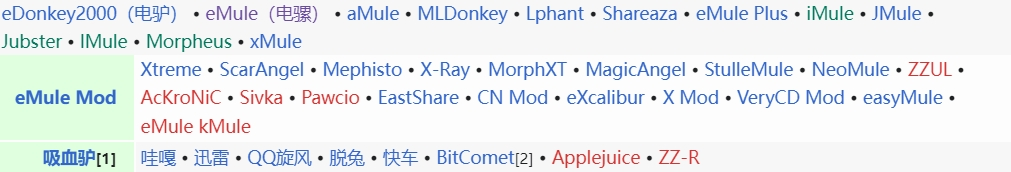
\includegraphics[width=1\textwidth]{Figures/eDonkey.png}
\caption{eDonkey协议的客户端}
\label{fig:eDonkey}
\end{figure}

\url{https://zh.wikipedia.org/wiki/EMule}
\url{https://www.ramonmillan.com/documentos/bibliografia/eMuleProtocolSpecification.pdf}

\section{Remote desktops}
\subsection{protocols}
远程控制协议指的是用于远程使用桌面计算机的协议或者技术标准。主流的远程控制协议包括远程帧缓冲(RFB)、远程桌面协议(RDP)、SPICE、独立计算体系结构(ICA)、PCoIP(PC over IP)等。

1.ICA协议:远程控制协议最早可以追溯到1989年,由Citrix公司开发了ICA协议,ICA协议不局限于任何单一平台,并规定了服务器和客户端之间传递数据的规范。Citrix ICA包括服务器软件组件、网络协议组件和客户端软件组件。如图\ref{fig:ICA}所示,ICA 协议在OSI模型的表示层运行,兼容大多数行业标准网络协议上,例如 TCP/IP、NetBEUI、IPX/SPX 和点对点协议(PPP)。它还运行在传输协议上,例如综合业务数字网 (ISDN)、帧中继和异步传输模式 (ATM)。用户可以通过拨号、局域网 (LAN)、广域网 (WAN) 或 Internet 连接访问在基于 ICA 的远程服务器上运行的标准 Windows 应用程序。应用程序可以从网页或 Windows 桌面启动,从而使 ICA 协议成为独立于平台的解决方案。

\begin{figure}[!htbp]
\centering
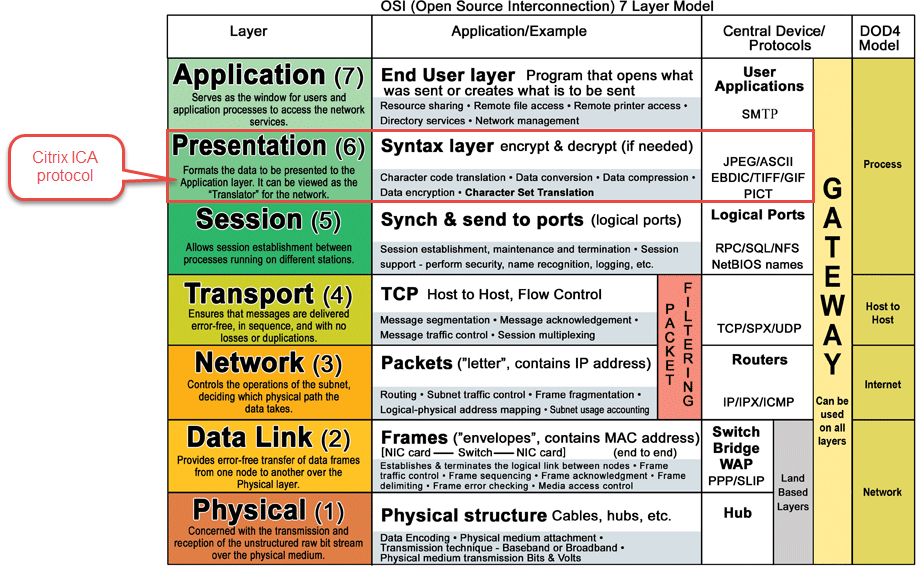
\includegraphics[width=1\textwidth]{Figures/ICA.png}
\caption{ICA协议}
\label{fig:ICA}
\end{figure}

\url{https://networkencyclopedia.com/independent-computing-architecture-ica/}

\url{https://pawelserwan.wordpress.com/2014/09/24/dive-into-citrix-ica-protocol-part1/}

2.RDP:Microsoft远程桌面协议(RDP)通过网络连接为服务器上运行的基于Windows的应用程序提供远程显示和输入功能。RDP基于和扩展了ITU T.120 系列协议,允许单独的虚拟通道从服务器传输设备通信和演示数据,以及加密的客户端鼠标和键盘数据,支持多达 64,000 个独立的通道进行数据传输和多点传输预配。RDP的底层协议如图\ref{RDP}所示。
\begin{figure}[!htbp]
\centering
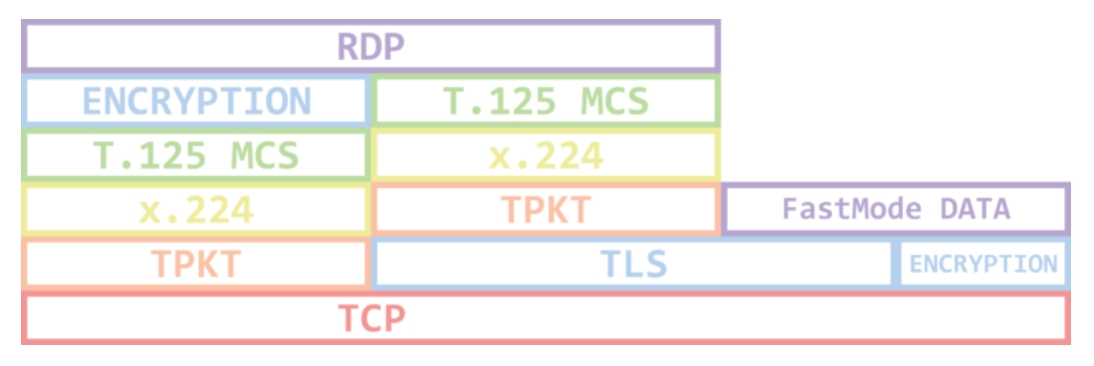
\includegraphics[width=1\textwidth]{Figures/RDP.png}
\caption{RDP协议栈}
\label{fig:RDP}
\end{figure}

\url{https://learn.microsoft.com/en-us/windows/win32/termserv/remote-desktop-protocol?source=recommendations}

3.RFB协议:RFB是一个用于远程访问图形用户接口的简单协议,VNC是基于此协议开发的。RFB适用于所有的桌面系统和应用,包括X11,Windows和Macintosh等。RFB协议的流程如图\ref{fig:RFB}所示。

\begin{figure}[!htbp]
\centering
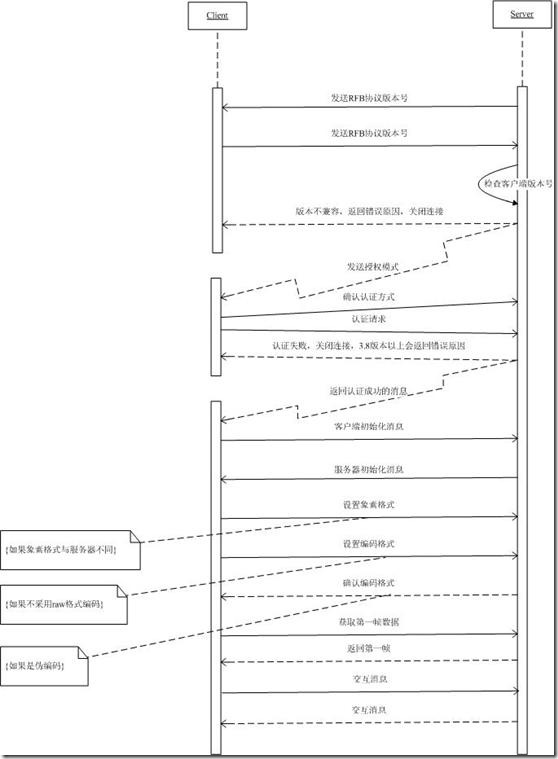
\includegraphics[width=1\textwidth]{Figures/RFB.png}
\caption{RFB协议流程图}
\label{fig:RFB}
\end{figure}

RFB的特点:(1)RFB协议是一个瘦客户协议,协议设计的重点是减小对客户端的要求。(2)RFB协议的客户端是“无状态”的。如果一个客户端和服务器断开了连接,稍后再一次连接到这台服务器上,用户的会话不会被关闭,状态会一直保持着。不同的客户端可以连接到同一个服务器上,在新的客户端上用户看到的是和原来的客户端上相同的图形用户接口。只要有合适的网络连接,用户就可以访问他个人的桌面应用,不论他走到哪里都可以连接到自己的会话上,而这些应用的状态可以一直保持着。

\url{https://www.cnblogs.com/szBeginner/p/7795307.html}

4.simple protocol for independent computing environment(SPICE)协议:SPICE协议是Redhat提出的一种远程桌面连接协议。该协议具有高可靠性和动态可移植性的特点。SPICE协议定义了一组协议消息,用于跨网络访问、控制和接收来自远程计算设备(例如键盘、视频、鼠标)的输入,并向它们发送输出。受控设备可以位于客户端和/或服务器的任一侧。此外,该协议还定义了一组调用,用于支持远程服务器从一个网络地址迁移到另一个网络地址。除了一个例外,传输数据的加密被排除在协议之外,以便在选择加密方法时具有最大的灵活性。

SPICE通信会话被分成多个通信通道,以便能够根据通道类型(例如 QoS 加密)控制消息的通信和执行,并在运行时添加和删除通信通道。当前协议定义中定义了以下通信通道:a)主通道,用作主要的SPICE会话连接; b)显示通道,用于接收远程显示更新; c)输入通道,用于发送鼠标和键盘事件; d)光标通道,用于接收指针形状和位置; e)播放通道,用于接收音频流;f)记录通道,用于发送音频捕获。SPICE协议的结构如图\ref{fig:Architecture-of-SPICE-protocol}所示。
\begin{figure}[!htbp]
\centering
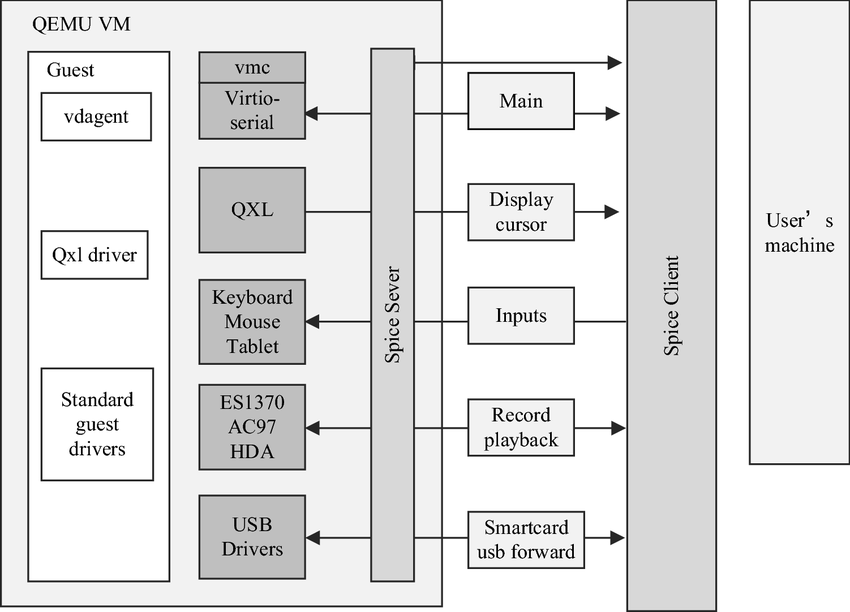
\includegraphics[width=1\textwidth]{Figures/Architecture-of-SPICE-protocol.png}
\caption{SPICE协议结构图}
\label{fig:Architecture-of-SPICE-protocol}
\end{figure}

\url{https://www.spice-space.org/spice-protocol.html}

5.PCoIP协议:PCoIP协议由Teradici开发,用于在远程访问服务器时压缩和解压缩图像和声音,并在硬件中实现。该协议有硬件和软件两种版本。2008年,VMware授权Teradici的PCoIP协议,并在VMware Horizon View中支持该协议。2013年,亚马逊授权PCoIP协议在AWS亚马逊工作区中使用。它帮助 Nutanix 在本地或混合云环境中部署工作站和虚拟桌面,并且可以通过 Microsoft Azure、Amazon Web Services 和 Google Computing Services 在公共云中找到它。PCoIP是一种基于UDP的协议,具有主机渲染、多编解码器和动态自适应功能。服务器上渲染的图像被捕获为像素,进行压缩和编码,然后发送到客户端进行解密和解压缩。根据图像的不同,使用不同的编解码器对发送的像素进行编码,因为压缩视频图像的技术与压缩文本的技术相比在有效性上不同。该协议还根据可用带宽动态调整其编码。在低带宽环境中,它使用有损压缩,快速传递高度压缩的图像,然后添加额外的数据来细化图像,这一过程被称为“构建到感知无损”。

\url{https://en.wikipedia.org/wiki/Teradici}

\subsection{Softwares}
1.VNC:VNC系统由客户端,服务端和一个协议组成。VNC默认使用TCP端口5900至5906,而JAVA的VNC客户端使用5800至5806。一个服务端可以在5900端口用“监听模式”连接一个客户端,使用监听模式的一个好处是服务端不需要设置防火墙。

基于VNC的派生软件:

(1)RealVNC
\begin{itemize}
\item[$\bullet$]The original developers. Out in the market the longest.
\item[$\bullet$]The free version lacks a lot of features which are included in other VNC clients and it not being actively developed. Not a good thing.
\item[$\bullet$]RealVNC provides remote control software which lets you see and interact with desktop applications across any network.
\item[$\bullet$]The software has a widespread user base from individuals to the largest multi-national companies. Founded by the original developers of VNC to promote, enhance and commercialise VNC.
\end{itemize}

(2)TightVNC
\begin{itemize}
\item[$\bullet$]Const Kaplinsky’s project to improve VNC’s compression between server and viewer. Good replacement for RealVNC, but graphic and performance is sluggish sometimes.
\item[$\bullet$]Does not allow remote copy and paste.
\item[$\bullet$]The project is being actively maintain, which is a plus.
\item[$\bullet$]TightVNC is a free remote control software package. With TightVNC, you can see the desktop of a remote machine and control it with your local mouse and keyboard, just like you would do it sitting in the front of that computer.
\end{itemize}

(3)UltraVNC
\begin{itemize}
\item[$\bullet$]A project to add in file transfer, chat messaging and NTLM authentication to VNC.
\item[$\bullet$]Based on experience, UltraVNC runs faster than the other two and has better graphics.
Has file transfer, faster connections, chat interface, etc
\item[$\bullet$]Allows you to copy and paste from your local computer to remote computer and vice versa
UltraVNC is a powerful, easy to use and free software that can display the screen of another computer (via internet or network) on your own screen. The program allows you to use your mouse and keyboard to control the other PC remotely. It means that you can work on a remote computer, as if you were sitting in front of it, right from your current location. If you provide computer support, you can quickly access your customer’s computers from anywhere in the world and resolve helpdesk issues remotely! With addons like SingleClick your customers don’t even have to pre-install software or execute complex procedures to get remote helpdesk support.
\end{itemize}

\url{https://blog.csdn.net/ayang1986/article/details/79537276}

2.RDP:RDP是由微软开发的专用协议,RDP 协议开启一个专用的网络通道,用于在连接的两台计算机(远程桌面和当前使用的计算机)之间来回发送数据。为此,它始终使用网络端口 3389。鼠标移动、击键、桌面显示和所有其他必要的数据利用 TCP/IP 并通过此通道发送,这是用于大多数种类的 Internet 流量的传输协议。RDP 也会加密所有数据,提升通过公共互联网连接的安全性。

集成RDP的软件:

(1)RDS

远程桌面服务,它是微软的桌面虚拟化解决方案的统称。它包括六个组件:RDCB,Remote Desktop Connection Broker,远程桌面连接代理、RDGW,Remote Desktop Gateway,远程桌面网关、RDWA,Remote Desktop Web Access,远程桌面 Web 访问、RDVH,Remote Desktop Virtualization Host,远程桌面虚拟化主机、RDSH,Remote Desktop Session Host,远程桌面会话主机及RDLS,Remote Desktop License Server,远程桌面授权服务器。

(2)Parallels RAS

Parallels RAS是Parallels生产的应用程序虚拟化软件,允许通过共享服务器或云系统中的单个设备访问Windows应用程序,于2014年由2X Software首次发布。使用Parallels RAS,Windows应用程序可以在通常无法运行它们的设备上使用,包括Macintosh计算机、移动设备和Google Chromebook。

(3)jump desktop

jump desktop是macOS上非常专业的远程桌面控制软件,可以帮助用户通过局域网或互联网安全可靠地连接到其他计算机。Jump Desktop支持全屏、文本粘贴复制、快捷键发送等功能,操作也非常简单,通过邮件关联即可帮助设备自动找到桌面并进行操作。

3.多协议集成

(1)RustDesk
\begin{itemize}
\item[$\bullet$]开源免费的远程桌面软件,开箱即用,无需任何配置。
\item[$\bullet$]您完全掌控数据,不用担心安全问题。
\item[$\bullet$]您可以使用我们的注册/中继服务器,或者自建,亦或者开发您的版本。
\end{itemize}

(2)Sunlgin
\begin{itemize}
\item[$\bullet$]跨平台连接-Windows、Mac、Linux、Android 之间互连,iOS 可远程以上设备。
\item[$\bullet$]极速流畅-使用 BGP 跨线路云服务器、多节点服务器及 H.264 智能视频模式。"网络稳定、远程流畅。
\item[$\bullet$]无人值守-随时远程访问和管理无人值守设备。
\end{itemize}

(3)TeamViewer
\begin{itemize}
\item[$\bullet$]历史-老牌远程桌面软件,即时连接,绝无拖延。
\item[$\bullet$]安全-TeamViewer 采用 256 位 AES 端到端加密、双因素身份验证及其他行业领先的安全功能,通过了SOC2、HIPAA/HITECH、ISO/IEC27001及IS0 9001:2015 认证,且符合 GDPR 的标准。
\item[$\bullet$]跨平台-TeamViewer 在总体覆盖率方面独步当世,覆盖范围囊括目前市场上 127 家制造商的移动设备、操作系统及 loT 设备,令竞争对手难以企及。
\item[$\bullet$]性能卓越-在可用性、图像质量及文件传输速度方面堪称同类产品中的翘楚;TeamViewer聘请了世界领先的独立质量保证公司 Qualitest 对其技术性能进行测试,并与竞争对手进行对比。 结果令人惊叹不已!
\end{itemize}

(4)ToDesk
\begin{itemize}
\item[$\bullet$]商业授权(个人免费)连接不限速连接不限速,支持设备数100个,支持点对点(P2P)连接模式。
\item[$\bullet$]遍布全国的网络节点。
\item[$\bullet$]SSL+ChaCha20 and Poly1305 端到端加密。
\end{itemize}

(5)AnyDesk
\begin{itemize}
\item[$\bullet$]访问与控制-AnyDesk高性能远程桌面软件实现无延迟的桌面分享、稳定的远程管理,以及设备之间快速安全的数据传输。
\item[$\bullet$]管理与定制-AnyDesk的功能并非一成不变。我们高度灵活的解决方案提供数不清的定制选项,适应任何 IT 管理员的需求。
\item[$\bullet$]安全与隐私-安全是我们的首要任务。AnyDesk的安全功能数不清,可以满足您的个人安全需求。
\item[$\bullet$]协作-AnyDesk延迟低,团队合作现在比以前更简单、更快。了解适合项目的最佳协作功能。
\end{itemize}

(6)Parsec
\begin{itemize}
\item[$\bullet$]难以置信的速度-Parsec 的专有技术消除了延迟。在几秒钟内访问您的硬件,延迟几乎为零。
\item[$\bullet$]响应式控制-插入键盘、鼠标、绘图板或游戏手柄,以无与伦比的输入精度和控制完成您的工作。
\item[$\bullet$]华丽的视频-在多台显示器上以鲜艳的色彩流式传输如丝般流畅的 60FPS UHD 交互式桌面视频。
\item[$\bullet$]加密对等连接-Parsec 将计算机锁定为仅限团队中的人员,并让他们直接连接。您的工作从不接触服务器。
\item[$\bullet$]高级工具和权限-自信地在您的组织中部署 Parsec:实施 SSO、设置会话持续时间,甚至为流添加水印。
\item[$\bullet$]团队管理-从单个管理仪表板添加和删除用户、组织组权限并处理帐单。
\item[$\bullet$]共享工作站-将计算机用于共同目的,并让团队成员按需访问它们。
\item[$\bullet$]访客访问-在有限的时间内安全地安排和邀请来自组织外部的用户。
\item[$\bullet$]即时协作-让团队成员一起工作,只需单击一个按钮,就任务提供反馈、专业知识和帮助。
\end{itemize}

\url{https://hexingxing.cn/remote-desktop-control/#TOP1%EF%BC%9ARustDesk}

\end{CJK}
\end{document}
